\begin{appendix}

\FloatBarrier
\section{Code repository}
All code used for this project is available at \href{https://github.com/ericludvigs/AST5220_Cosmology_Project}{this Github repository}.
The src folder contains the numerical C++ code. Calculated results are in csv-files found under the results folder. Presentation is handled by Python scripts per milestone, in the respective Milestone X folders. Produced plots are saved to a Plots folder under each Milestone.

\FloatBarrier
\section{Milestone I, extra plots}\label{app:milestone_1_extra_plots}

Evolution of some physical quantities in figs. \ref{fig:milestone_1_H_prime_of_x} and \ref{fig:milestone_1_eta_of_x}.

\begin{figure}[h!tb]
\centering
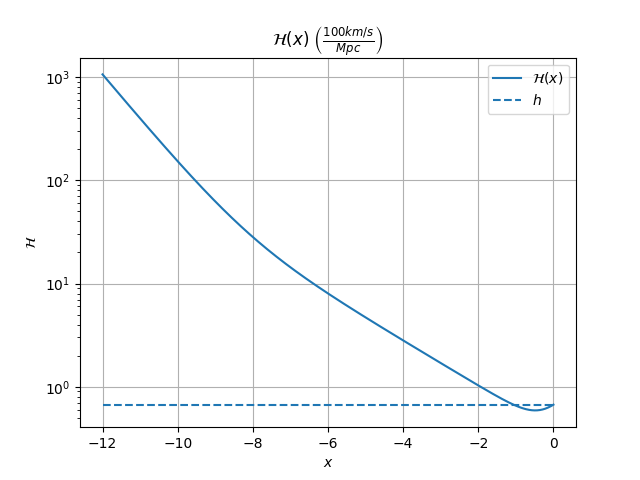
\includegraphics[width=0.4\textwidth]{../Milestone 1/Plots/H_prime_of_x.png}
\caption{Direct plot of $\mathcal{H}$. For reference the current accepted value of $h$ is plotted, which intercepts the plot as expected at $x=0$. We see the expected steady falloff with a slight change in steepness as the universe becomes matter dominated, and a reversal in the size of $H$ as the universe becomes dominated by dark energy.}
\label{fig:milestone_1_H_prime_of_x}
\end{figure}

\begin{figure}[h!bt]
\centering
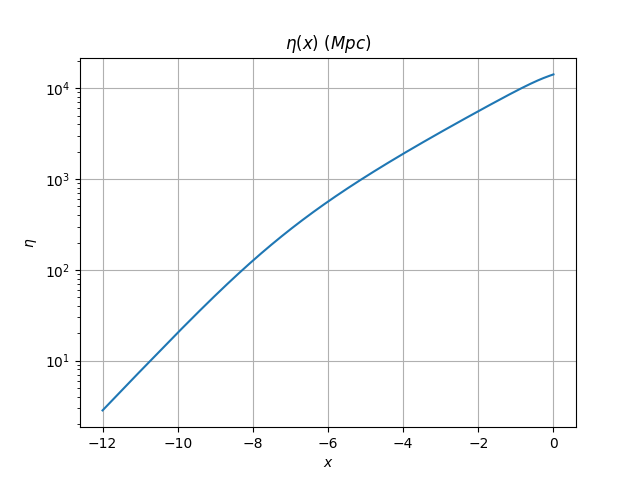
\includegraphics[width=0.4\textwidth]{../Milestone 1/Plots/eta_of_x.png}
\caption{Direct plot of the conformal time. Relates to cosmic horizons, which expand slowly in the radiation dominated era.}
\label{fig:milestone_1_eta_of_x}
\end{figure}

Histograms of parameter distribution in fig. \ref{fig:milestone_1_appendix_histograms}.

\begin{figure*}[h!tb]
\centering
    \begin{subfigure}[t!]{0.4\textwidth}
    \centering
    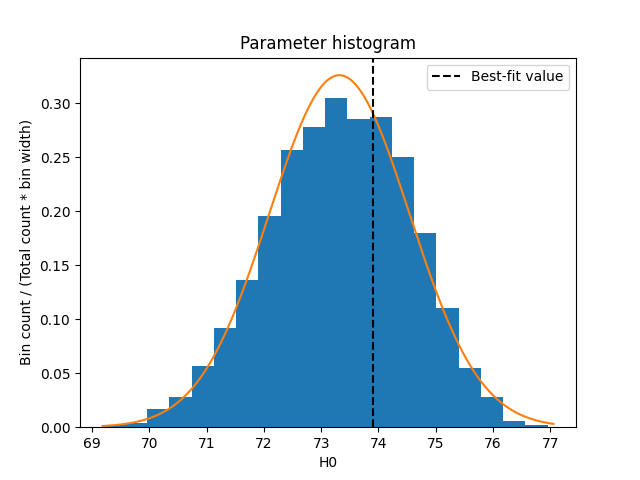
\includegraphics[width=1.0\textwidth]{../Milestone 1/Plots/H0_histogram.png}
    \caption{Accepted samples for $H_0$.}
    \label{fig:milestone_1_H0_histogram}
    \end{subfigure}
    %\hfill
    \begin{subfigure}[t!]{0.4\textwidth}
    \centering
    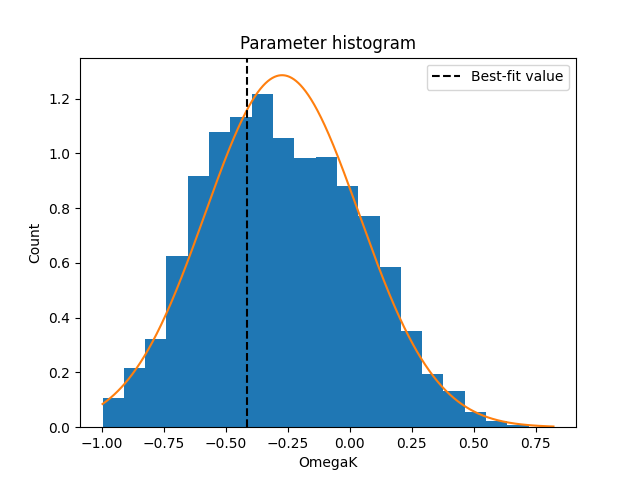
\includegraphics[width=1.0\textwidth]{../Milestone 1/Plots/OmegaK_histogram.png}
    \caption{Accepted samples for $\Omega_K$.}
    \label{fig:milestone_1_OmegaK_histogram}
    \end{subfigure}
    \hfill
    %\hfill
    \begin{subfigure}[b!]{0.4\textwidth}
    \centering
    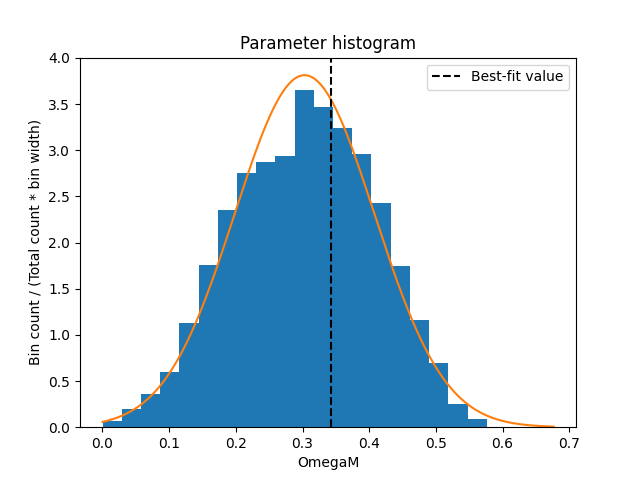
\includegraphics[width=1.0\textwidth]{../Milestone 1/Plots/OmegaM_histogram.png}
    \caption{Accepted samples for $\Omega_M$.}
    \label{fig:milestone_1_OmegaM_histogram}
    \end{subfigure}
    \begin{subfigure}[b!]{0.4\textwidth}
    \centering
    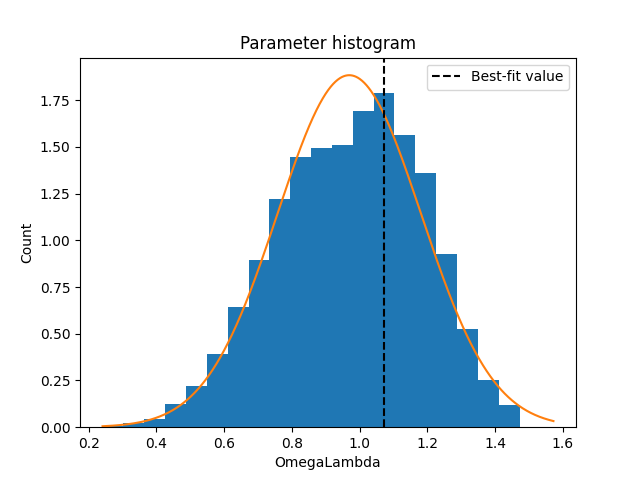
\includegraphics[width=1.0\textwidth]{../Milestone 1/Plots/OmegaLambda_histogram.png}
    \caption{Accepted samples for $\Omega_\Lambda$.}
    \label{fig:milestone_1_OmegaLambda_histogram}
    \end{subfigure}
\caption{Histogram of accepted samples from the MCMC, with a simple gaussian function with the same mean and standard deviation overplotted. Sampling covers a suitably random range and should be a good representation of possible parameter values. The final best-fit values are indicated.}
\label{fig:milestone_1_appendix_histograms}
\end{figure*}

%\FloatBarrier
\section{Milestone II, extra math}
Definitions to support Peebles equation (\ref{eq:peebles_equation}):

\boxed{
\begin{aligned}\label{eq:peebles_quantities_definition}
C_r(T_b) &= \frac{\Lambda_{2s\rightarrow1s} + \Lambda_{\alpha}}{\Lambda_{2s\rightarrow1s} + \Lambda_{\alpha} + \beta^{(2)}(T_b)}, \enspace \text{[dimensionless]}\\
H &,  \enspace \text{[\unit{1/s}]}\\
\Lambda_{2s\rightarrow1s} &= 8.227, \enspace \text{[\unit{1/s}]}\\
\Lambda_{\alpha} &= H\frac{(3\epsilon_0)^3}{(8\pi)^2 c^3 \hbar^3 n_{1s}}, \enspace \text{[\unit{1/s}]}\\
n_{1s} &= (1-X_e)n_H, \enspace \text{[\unit{1/m^3}]}\\
n_H &= (1-Y_p) n_b \approx (1-Y_p) \frac{3H_0^2\Omega_{b0}}{8\pi G m_H a^3}, \enspace \text{[\unit{1/m^3}]}\\
\beta^{(2)}(T_b) &= \beta(T_b) e^{\frac{3\epsilon_0}{4 k_b T_b}}, \enspace \text{[\unit{1/s}]}\\
\beta(T_b) &= \alpha^{(2)}(T_b) \left(\frac{m_e k_b T_b}{2\pi \mathbf{\hbar}^2}\right)^{3/2} e^{-\frac{\epsilon_0}{k_b T_b}}, \enspace \text{[\unit{1/s}]} \\
\alpha^{(2)}(T_b) &= \frac{8}{\sqrt{3\pi}} c \sigma_T \sqrt{\frac{\epsilon_0}{k_b T_b}}\phi_2(T_b), \enspace \text{[\unit{m^3/s}]}\\
\phi_2(T_b) &= 0.448\ln\left(\frac{\epsilon_0}{k_b T_b}\right), \enspace \text{[dimensionless]}\\
\sigma_T &= \frac{8\pi}{3} \left(\frac{\alpha \hbar c}{m_e c^2}\right)^2, \enspace \text{[\unit{m^2}]}\\
    &\begin{aligned}
    \alpha \simeq \frac{1}{137.0359992} \enspace &\text{[dimensionless,}\\
    &\text{{fine-structure constant}]}
    \end{aligned}
\end{aligned}
}

\FloatBarrier
\section{Milestone III, extra math}

Initial conditions for \ref{eq:milestone_3_ode_initial_conditions}:

\begin{equation}\label{eq:milestone_3_ode_initial_conditions}
\boxed{
\begin{aligned}
\Psi &= -\frac{1}{\frac{3}{2} + \frac{2f_\nu}{5}}\\
\Phi &= -(1+\frac{2f_\nu}{5})\Psi \\
\delta_{\rm CDM} &= \delta_b = -\frac{3}{2} \Psi \\
v_{\rm CDM} &= v_b = -\frac{ck}{2\mathcal{H}} \Psi\\
&\text{Photon multipoles:}\\
\Theta_0 &= -\frac{1}{2} \Psi \\
\Theta_1 &= +\frac{ck}{6\mathcal{H}}\Psi \\
\Theta_2 &= -\frac{20ck}{45\mathcal{H}\tau^\prime} \Theta_1 \quad\quad \textrm{(without polarization)} \\
\Theta_\ell &= -\frac{\ell}{2\ell+1} \frac{ck}{\mathcal{H}\tau^\prime} \Theta_{\ell-1}\\
\end{aligned}
}
\end{equation}

\end{appendix}
